\begin{center}{ \bf  ТОПОЛОГИЯ СЛОЕНИЙ ЛИУВИЛЛЯ \\
ФАЗОВОГО ПРОСТРАНСТВА СЛУЧАЯ \\
КОВАЛЕВСКОЙ НА АЛГЕБРЕ ЛИ so(4)}\\
{\it В.А. Кибкало } \\
(МГУ им. М.В.\,Ломоносова; {\it slava.kibkalo@gmail.com} )
Работа выполнена при поддержке РНФ, грант  17-11-01303
\end{center}
\addcontentsline{toc}{section}{Кибкало В.А.}


\textbf{1.} Рассмотрим вполне интегрируемую по Лиувиллю система $v = \textrm{sgrad} H$ на фазовом пространстве.

На симплектическом $(M^4, \omega)$ такие системы имеют два инволютивных, функционально независимых первых интеграла $H, K$ с полными потоками. Фазовое пространство расслаивается на двумерные неособые торы и особые слои --- совместные уровни первых{ интегралов. Почти все траектории реализуют условно-периодическую обмотку тора.

В работах А.Т. Фоменко и его школы исследовались свойства таких слоений на трехмерных поверхностях $Q^3$ [1]. Согласно теореме Фоменко-Цишанга, два слоения на неособых $Q^3_1$~и~$Q^3_2$ эквивалентны $\Leftrightarrow$ совпадает их инвариант Фоменко-Цишанга. Он является графом с числовыми метками $(r, \varepsilon, n)$, вершины которого соответствуют особым слоям, а ребра --- семействам неособых. Лиувиллев анализ (их вычисление) для классических систем проводился многими авторами.

\textbf{2.}  Гамильтоновы системы порождают динамические системы на орбитах коприсоединенного представления алгебр Ли. Ряд новых систем получается из классических "возмущением"\ гамильтониана и скобки Ли--Пуассона. Например, И.В.\,Комаров [2] вложил (при $\varkappa =0$) случай Ковалевской на $\textrm{e}(3)$  в семейство динамических систем на пучке алгебр Ли $\textrm{e}(3,1)-\textrm{e}(3)-\textrm{so}(4)$ на $\mathbb{R}^6(\mathbf{J}, \mathbf{x})$ со скобками Пуассона--Ли: %(\ref{Eq:Poisson_bracket}):
%\begin{equation} \label{Eq:Poisson_bracket}
\[\{J_i, J_j\} =
\varepsilon_{ijk}J_k, \quad \{J_i, x_j\} = \varepsilon_{ijk}x_k,
\quad \{x_i, x_j\} = \varkappa \varepsilon_{ijk}J_k, \]%\end{equation}
$\varepsilon_{ijk} = sgn(\{123\} \rightarrow \{ijk\})$. При  $\varkappa>0$ имеем алгебру $\textrm{so}(4)$. Орбита является совместным уровнем функций Казимира
%
\[f_1 = (x_1^2 + x_2^2 + x_3^2) + \varkappa (J_1^2 +J_2^2 +J_3^2),
\qquad  f_2 = x_1 J_1 + x_2 J_2 +x_3 J_3.\]
%
Гамильтониан $H$ и дополнительный интеграл $K$ имеют вид
%
\[H = J_1^2 + J_2^2 + 2J_3^2 + 2 c_1 x_1, \]
\[K = (J_1^2 - J_2^2-2c_1 x_1 + \varkappa
c_1^2)^2 + (2J_1 J_2 - 2 c_1 x_2)^2.\]

%
\textbf{3.} При $\varkappa >0$ автором классифицированы слоения неособых изоэнергетических $Q^3_{a,b,h}$ $=\{f_1=a,f_2=b,H=h\}.$

\textbf{Теорема~1.}{
1) В системе Ковалевской на so(4) существует ровно $27$ классов $L_1, \dots L_{27}$ лиувиллево неэквивалентных слоений на связных компонентах неособых $Q^3_{a, b, h}$.%=\{f_1=a, f_2=b, H=h\}$.

2) $\mathbb{R}^3_{a, b, h}$ разбито на $54$ связных открытых множества с фиксированным классом слоения на $Q_{a, b, h}$ и особое $\mathbb{A}^2$.
}

Эквивалентность слоений двух систем на $Q^3$ означает совпадение замыканий их решений при данных энергиях.

\textbf{Теорема~2.}{
Следующие слоения интегрируемых систем эквиваленты слоениям $L_i$ на $Q^3_{a, b, h}$ Ковалевской на $\mathrm{so}(4)$

1) случай Ковалевской на $\mathrm{e}(3)$  моделируется полностью:
$A,\, ...\, ,J$ (см. [3]) эквивалентны $L_i,\, i \in \{1, 12, 3, 4, 15, 27, 24, 20, 24, 18\}$, %L_{12}, L_3, L_4, L_{15}, L_{27}, L_{24}, L_{20}, L_{24}, L_{18}$,

2) Ковалевская--Яхьи: $h_{10}$ и $h_{2}$ эквивалентны $L_{23}$ и  $L_2$,

3) Клебш:  $1, 2, 6, 7$ эквивалентны $L_1, L_2, L_9, L_{10}$,

4) Соколов на $\mathrm{e}(3)$: $A, B, F$ эквивалентны $L_1, L_2, L_4$,

5) интегрируемые биллиарды в софокусных квадриках со склейками по выпуклым и невыпуклым дугам границы:
$A_0', A_2, A_1, A_0, \Delta_{\alpha}(A_1+A_1)$ (см. [5])  моделируют $L_1, L_2, L_6, L_8, L_7$.
}

%\begin{center}
%\end{center}
%\verb"\eqno"
\begin{figure}[!htb]
%
\begin{center}
\minipage{0.75\textwidth}
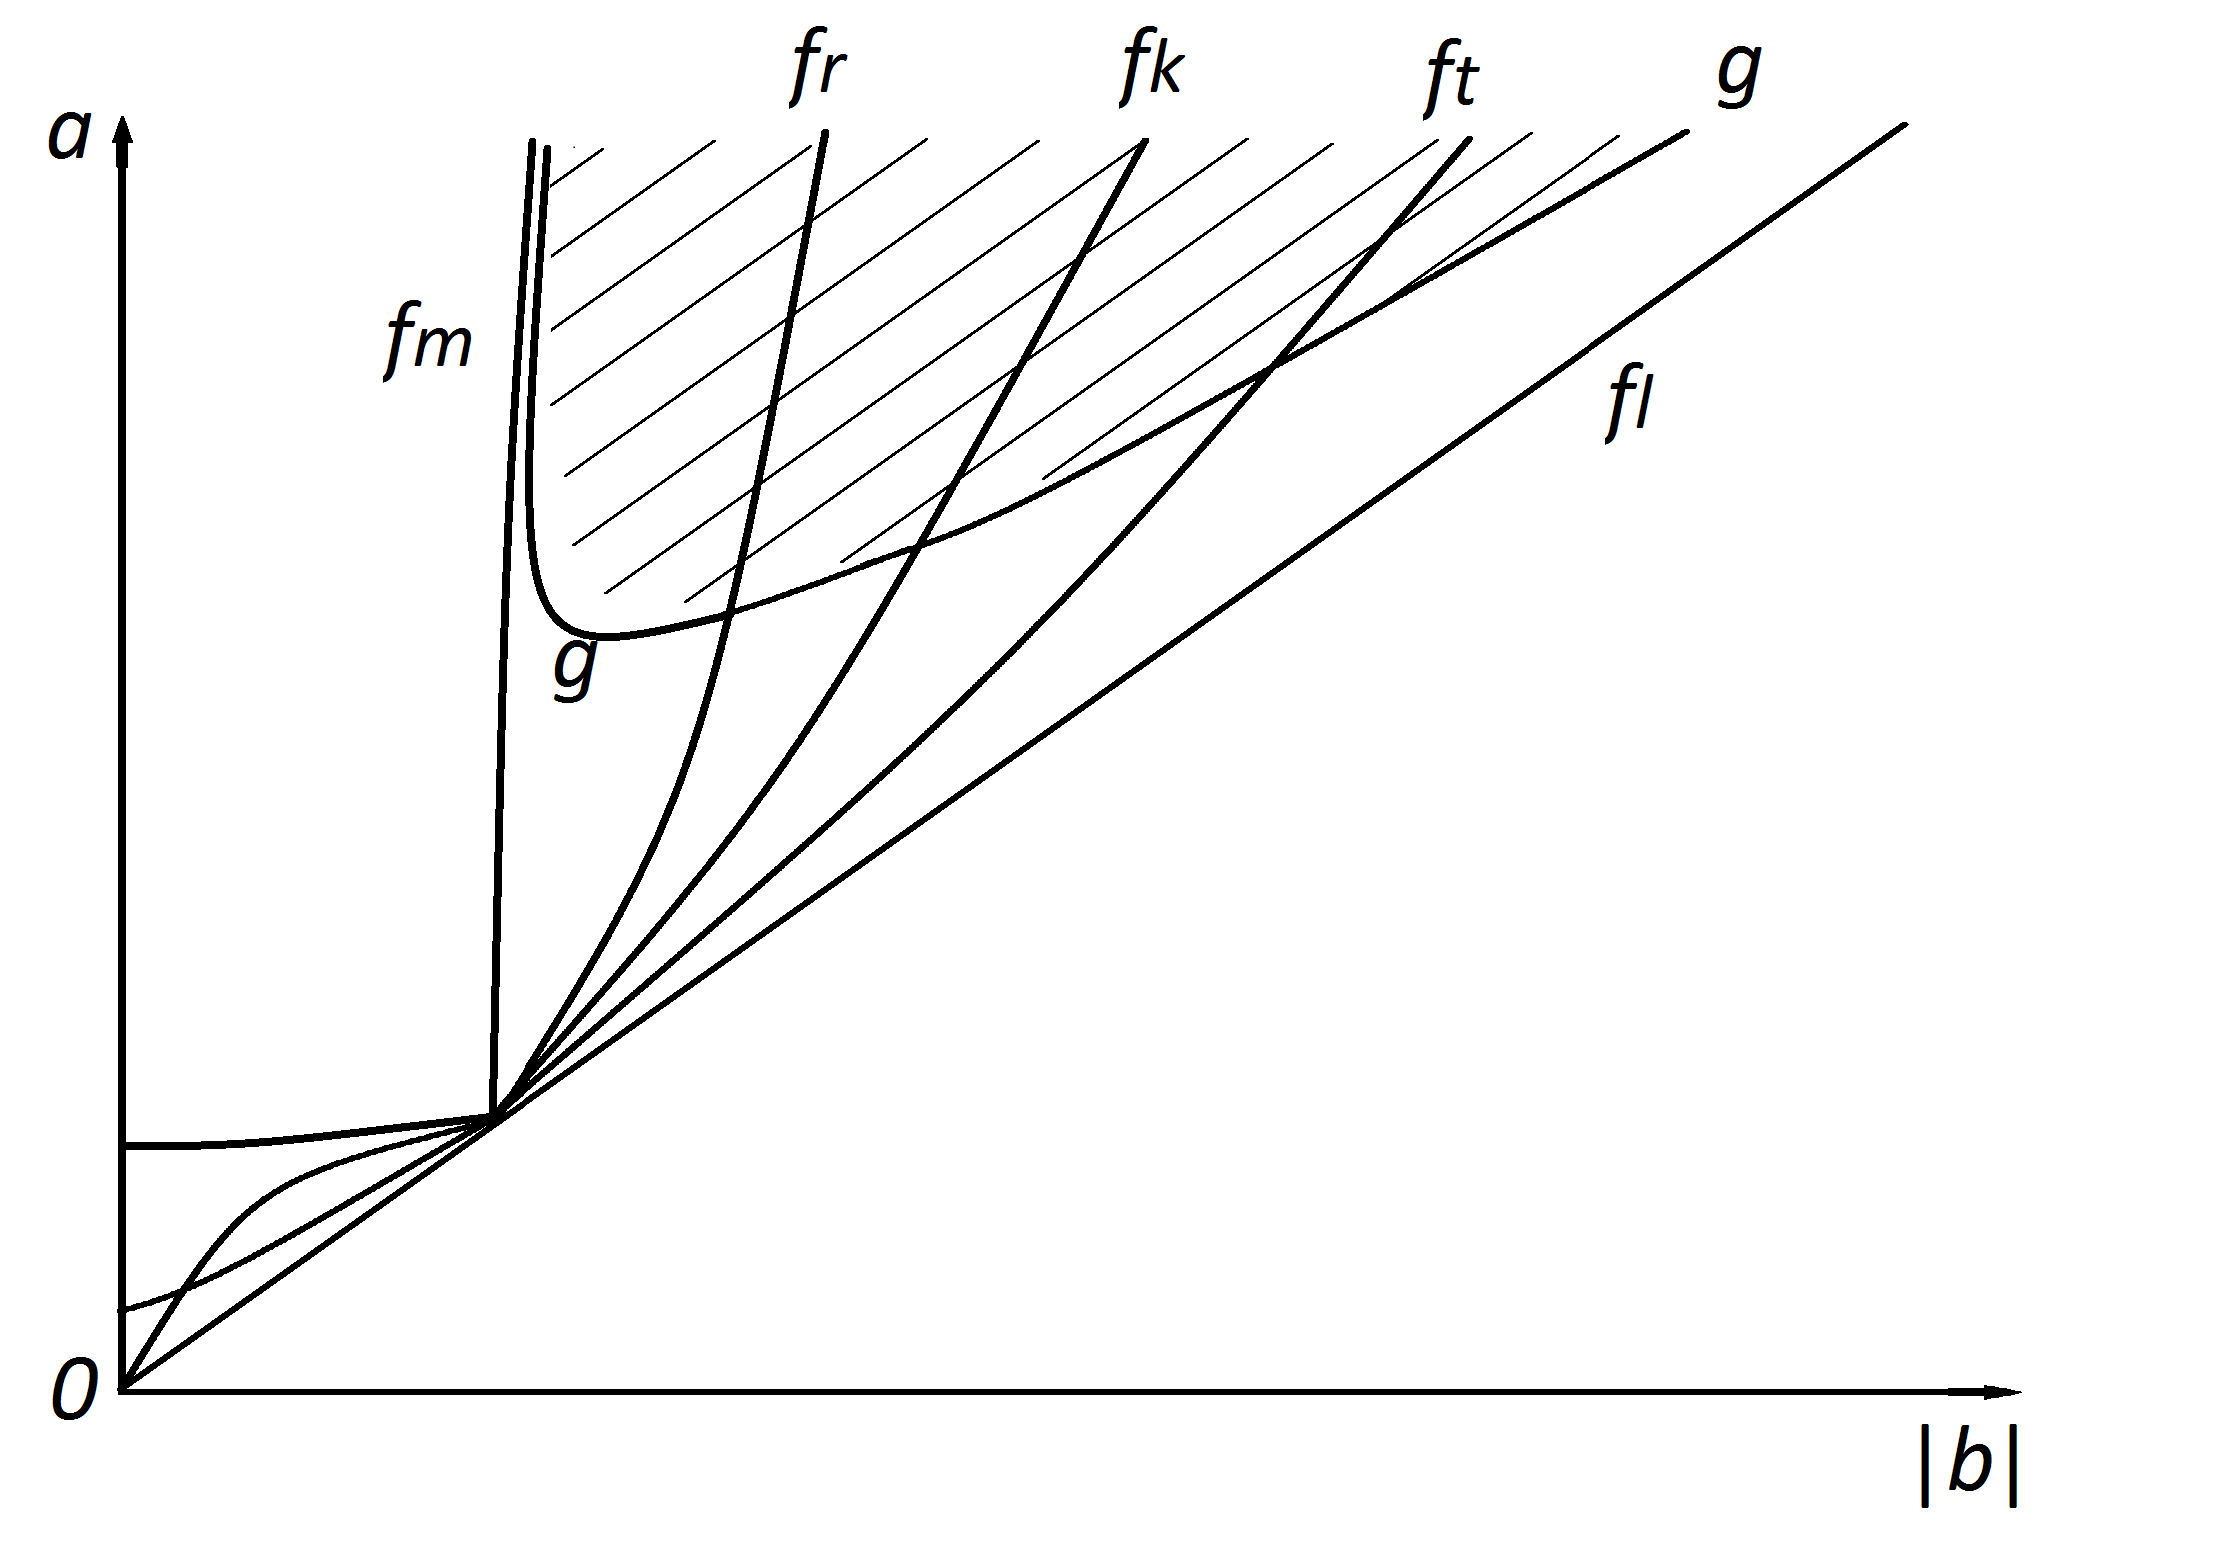
\includegraphics[width=\linewidth]{Kibkalo_vzms_18_pic}
   \caption{Cлучай $\mathrm{e}(3)$ ``вложен'' в случай $\mathrm{so}(4)$.}
\endminipage
\end{center}
\end{figure}


Каждая орбита $(a, b)$ задается значениями $f_1, f_2$, ей соответствует бифуркационная диаграмма отображения момента $\Sigma$ ([4]).
При $\varkappa >0$ для орбит $(a, b)$ c $a >g(b)$ особые точки $\Sigma$, не встречавшиеся при $\varkappa = 0$,~лежат в области $\{h > h_0(a, b)\}$, а остальные --- в $\{h < h_0(a, b)\}$.
Т.е. случай Ковалевской с $\varkappa =0$ в $a, b >0$ можно послойно отождествить с системой $\varkappa >0 \{a >g(b), h < h_0(a, b)\}$.



\smallskip \centerline{\bf Литература}\nopagebreak

1. {\it Болсинов А.В., Фоменко А.Т.} Интегрируемые гамильтоновы системы. Геометрия, топология, классификация. Ижевск.: Издат. дом ``Удмурт. ун-т'', 1999.

2. {\it Комаров И.В. } Базис Ковалевской для атома водорода. ТМФ 1981. {\bf47} \No~1. 67--72.


3. {\it Болсинов А.В., Рихтер П.Х., Фоменко А.Т.} Метод круговых молекул и топология волчка Ковалевской. Матем. сб. 2000. {\bf191}, \No~2. 3--42.

4. {\it Козлов И.К.} Топология слоения Лиувилля для интегрируемого случая Ковалевской на алгебре Ли so(4).  Матем. сб. 2014. {\bf205}, \No~4. 79--120.

5. {\it Ведюшкина В.В. } Слоение Лиувилля невыпуклых топологических биллиардов. ДАН 2018. {\bf418} \No~1.


